\documentclass[12pt]{article}
\usepackage{graphicx}
\usepackage{amsmath}

\begin{document}
CSCI-4100 Assignment 5\\
Yichuan Wang \\
RIN:661414395\\\\

EXERCISES\\
2.8\\
(a)$\overline{g}$ is a average function from $g_1...g_k$ derived from many datasets, and these many $g_1...g_k$ belong to $H$. Since average function is a form of linear combination, $\overline{g}$ must be in $H$.

(b)A model that contains two hypotheses, one constantly gives $-1$, the other constantly gives $+1$. If the  datasets gives $P[g_1=h_1=+1]=0.5$ and $P[g_2=h_2=-1]=0.5$, the expectation of $g$ is 0, which is not in the model.

(c)It can either be a binary function or not a binary function. It is possible that the model contains only one hypothesis so that $\overline{g}$ is always a binary function. However, when $\overline{g}$ is obtained by taking average of multiple functions, it is possible that fraction occurs during the division process for calculating average.

PROBLEMS\\
2.14 \\
(a) A hypothesis set $H_n$ with $d_{VC}$ indicates that $H_n$ can shatter at most $d_{VC}$ data points; therefore H can provide at most $K\times2^{d_{VC}}$ dichotomies before each sub hypothesis set reach its breakpoint. Since $K\times 2^{d_{VC}} \leq 2^{K\times d_{VC}}$ for K being a positive integer, $d_{VC}(H)\leq K\times d_{VC}$, and therefore $d_{VC}(H)< K\times (d_{VC}+1)$\\\\
(b) For $l$ data points, a hypothesis set $H$ with $d_{VC}$ can give at most $l^{d_{VC}}+1$ dichotomies. In this case, a $H$ with $H_1...H_K$ (each has $d_{VC}$) can give at most $Kl^{d_{VC}}+K$ dichotomies if all $H_1...H_k$ give their distinct $l^{d_{VC}}+1$ dichotomies, and formally this is (inequality 1) $$m_H(l)\leq Kl^{d_{VC}}+K$$
If we assume $l$, $d_{VC}$ and $K$ are all positive integers, we can conclude that $K\times l^{d_{VC}}\geq K$. And therefore we can derive the inequality 2: $$2Kl^{d_{VC}}\geq Kl^{d_{VC}}+K$$
We are given the inequality 3: $$2^l>2Kl^{d_{VC}} $$
Consider inequality 1,2 and 3, we can conclude $2^l> m_H(l)$, which implies $2^l\geq m_H(l)$.
By definition, $2^l\geq m_H(l)$ means $d_{VC}(H)\leq l$, and therefore we proved $d_{VC}(H)\leq l$.\\\\
(c)\\
$$2^{7(d_{VC+K})log_2(K\times d_{VC})}>2K(7(d_{VC+K})log_2(K\times d_{VC}))^{d_{VC}}$$
$$(K\times d_{VC})^{7(d_{VC}+K)}>2K(7(d_{VC+K})log_2(K\times d_{VC}))^{d_{VC}}$$
Taking the $log_2$ for both side we get inequality 1:
$$7(d_{VC}+K)log_2(Kd_{VC})>1+log_2(K)+7log_2(d_{VC})+d_{VC}log_2(d_{VC}+K)+d_{VC}log_2log_2(Kd_{VC})$$

We have following inequalities being trivially true if we assume $K>1$ and $d_{VC}> 1$:
$$d_{VC}log_2(Kd_{VC})>d_{VC}log_2log_2(Kd_{VC})$$
$$d_{VC}log_2(Kd_{VC})>1$$
$$7Klog_2(Kd_{VC}>7log_2(d_{VC}))$$
$$d_{VC}log_2(Kd_{VC})>log_2(K)$$
$$d_{VC}log_2(Kd_{VC})\geq d_{VC}log_2(d_{VC}+K)$$

The sum of the left side of these inequalities is the left side of inequality 1, and the sum of right side of these inequalities is the right side of inequality 1. In these case inequality 1 holds, indicating that the inequality in 2.14(b) is satisfied with $l=7(d_{VC}+K)log_2(Kd_{VC})$. Thus $$d_{VC}(H)\leq min(K(d_{VC}+1),7(d_{VC}+K)log_2(Kd_{VC}))$$
2.15\\
(a) A simple 2D monotonic classifier can be $h(x_1,x_2) = sign(x_1+x_2)$. When $x_{1i}\geq x_{1i+1}$ and $x_{2i}\geq x_{2i+1}$, $sign(x_{1i}+x_{2i})\geq sign(x_{1i+1}+x_{2i+1})$. The graph is shown below:\\
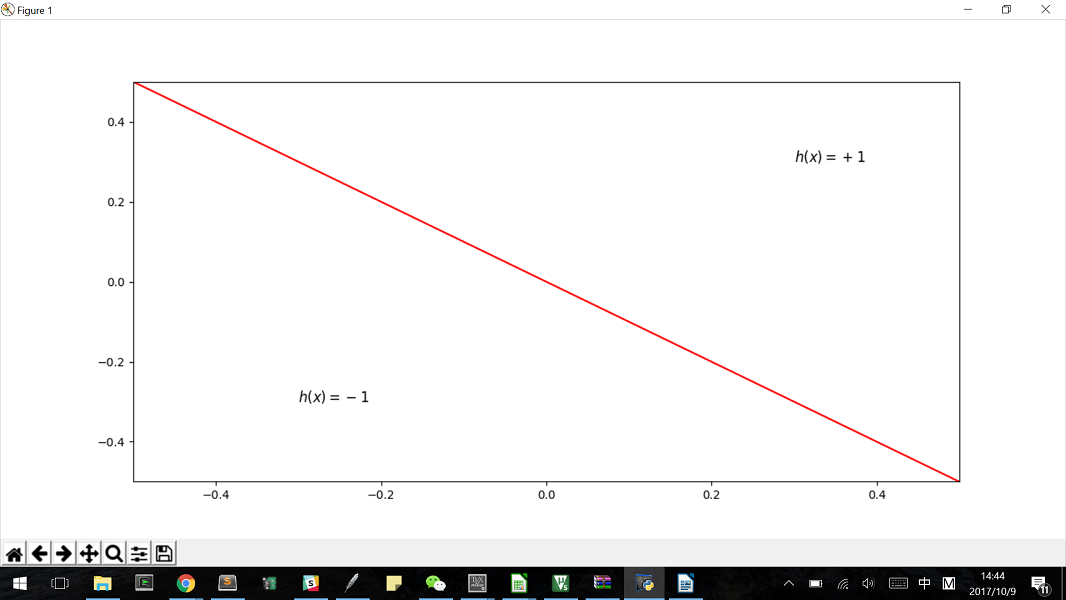
\includegraphics[scale=0.6]{monotonic}\\


(b) The VC dimension is infinity. Monotonic classifier means if $x_1\geq x_2$ then $h(x_1)\geq h(x_2)$. In this case if we have two data points such that $x1>x2$ and $h(x_2)=+1$, then we cannot implement $h(x_1)=-1$. However, if we place our data points according to the hint, that we place our point by increasing the first component and decreasing the second component of the previous point, we get a dataset in which no data point is greater than another. In this case our monotonic classier is not constrained any more; it can make any $h(x_n)$ either larger or smaller than any other $h(x_m)$, and thus it can classify any data points as +1 or -1 regardless of other data points. In this case these N data points can be shattered. Since we can place any number of data points according to this rule (the hint), the monotonic classifier can shatter any number of data points, and thus $d_{VC}=\infty$.\\ 
2.24
(a) The $\overline{g}$ is calculated as following:
$$\overline{g} = \frac{1}{2}\frac{1}{2} \int_{-1}^1\int_{-1}^1 (x_1+x_2)x-x_1x_2  dx_1dx_2$$
$$\overline{g} = \frac{1}{2}\frac{1}{2} \int_{-1}^1 \frac{x_1^2}{2}+x_2x-\frac{x_1^2}{2}x_2  \big|^1_{-1} dx_2$$
$$\overline{g} = \frac{1}{2}\frac{1}{2} \int_{-1}^1 x_2xdx_2$$
$$\overline{g} = \frac{1}{2}\frac{1}{2} \frac{x_2^2x}{2} \big|^1_{-1}$$
$$\overline{g} = 0$$
(b) Iteratively generate dataset D containing two random points in range [-1,1]. For each iteration, fit a line (output g) through points ($x_1$,$x_1^2$) and ($x_2$,$x_2^2$). Calculate $E_{out}$ for each iteration and average them to get $E[E_{out}]$ after N iterations. ($N>1000$)

After N iterations calculate $\overline{g}$ using previously generated N $g$ functions, and calculate $var$ using this $\overline{g}$ with respect to previously generated $g$ functions.

Calculate $bias$ using calculated $\overline{g}$ and target function $f(x)$.

Compare $E[E_{out}]$ with $bias+var$.\\\\
(c)
The following is the result of 5000 iterations:
$$\overline{g} = -0.0079x+0.0009$$
$$E_{out}=0.5288$$
$$var=0.3294$$
$$bias=0.1976$$
$$bias+var=0.5270$$
Graph:(blue line is f(x), red line is $\overline{g}$)\\
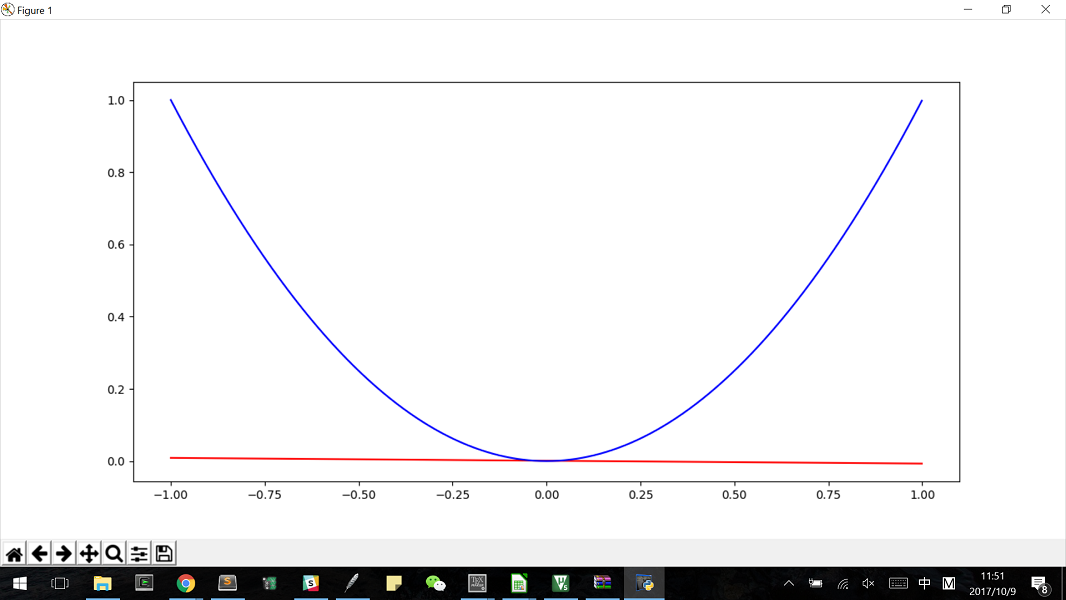
\includegraphics[scale=0.6]{graph}\\
(d)
$$bias = (\overline{g}(x)-f(x))^2=\frac{1}{2}\int_{-1}^{1}x^4dx=\frac{1}{5}$$
$$var = E_x[E_D[(g^{(D)}(x)-\overline{g}(x))^2]]$$
$$var = \frac{1}{2}\int_{-1}^1 \frac{1}{2} \frac{1}{2}\int_{-1}^1\int_{-1}^1 ((x_1+x_2)x-x_1x_2)^2 dx_1dx_2dx$$
$$var = \frac{1}{8}\int_{-1}^1\int_{-1}^1\int_{-1}^1 (x_1+x_2)^2x^2-2(x_1x_2(x_1+x_2))x+(x_1x_2)^2 dx_1dx_2dx$$
$$var = \frac{1}{8}\int_{-1}^1\int_{-1}^1\int_{-1}^1 (x_1^2+2x_1x_2+x_2^2)x^2-2(x_1^2x_2+x_1x_2^2)x+(x_1x_2)^2 dx_1dx_2dx$$
$$var = \frac{1}{8}\int_{-1}^1\int_{-1}^1 (\frac{x_1^3}{3}+x_1^2x_2+x_2^2)x^2-2(\frac{x^3}{3}x_2+\frac{x_1^2}{2}x_2^2)x+\frac{x_1^3}{3}x_2^2 \big|^1_{-1}dx_2dx$$
$$var = \frac{1}{8}\int_{-1}^1\int_{-1}^1 (\frac{2}{3}+x_2^2)x^2-\frac{4}{3}x_2+\frac{2}{3}x_2^2 dx_2dx$$
$$var = \frac{1}{8}\int_{-1}^1 (\frac{2}{3}+\frac{x_2^3}{3})x^2-\frac{4}{3}x_2^2+\frac{2}{9}x_2^3 \big|^1_{-1}dx$$
$$var = \frac{1}{8}\int_{-1}^1 (\frac{2}{3}+\frac{2}{3})x^2+\frac{4}{9}dx$$
$$var = \frac{1}{8}(\frac{2}{3}+\frac{2}{9})x^3+\frac{4}{9}x) \big|^1_{-1}$$
$$var = \frac{1}{8}(\frac{16}{9}+\frac{8}{9})=\frac{1}{3}$$
$$E[E_{out}]=bias+var=\frac{1}{5}+\frac{1}{3}=\frac{8}{15}$$
\end{document}